\documentclass[../DefinizioneDiProdotto_v3.0.0.tex]{subfiles}

\begin{document}

\section{Diagrammi di attività}
In questa sezione viene descritta e rappresentata tramite un diagramma di attività UML la sequenza di azioni del FlowModule.

\subsection{FlowModule}
Nel seguente diagramma viene riportato il flusso di azioni che l'AV esegue ogni volta che riceve una risposta ad una domanda.

\begin{figure}[!h]
	\centering
	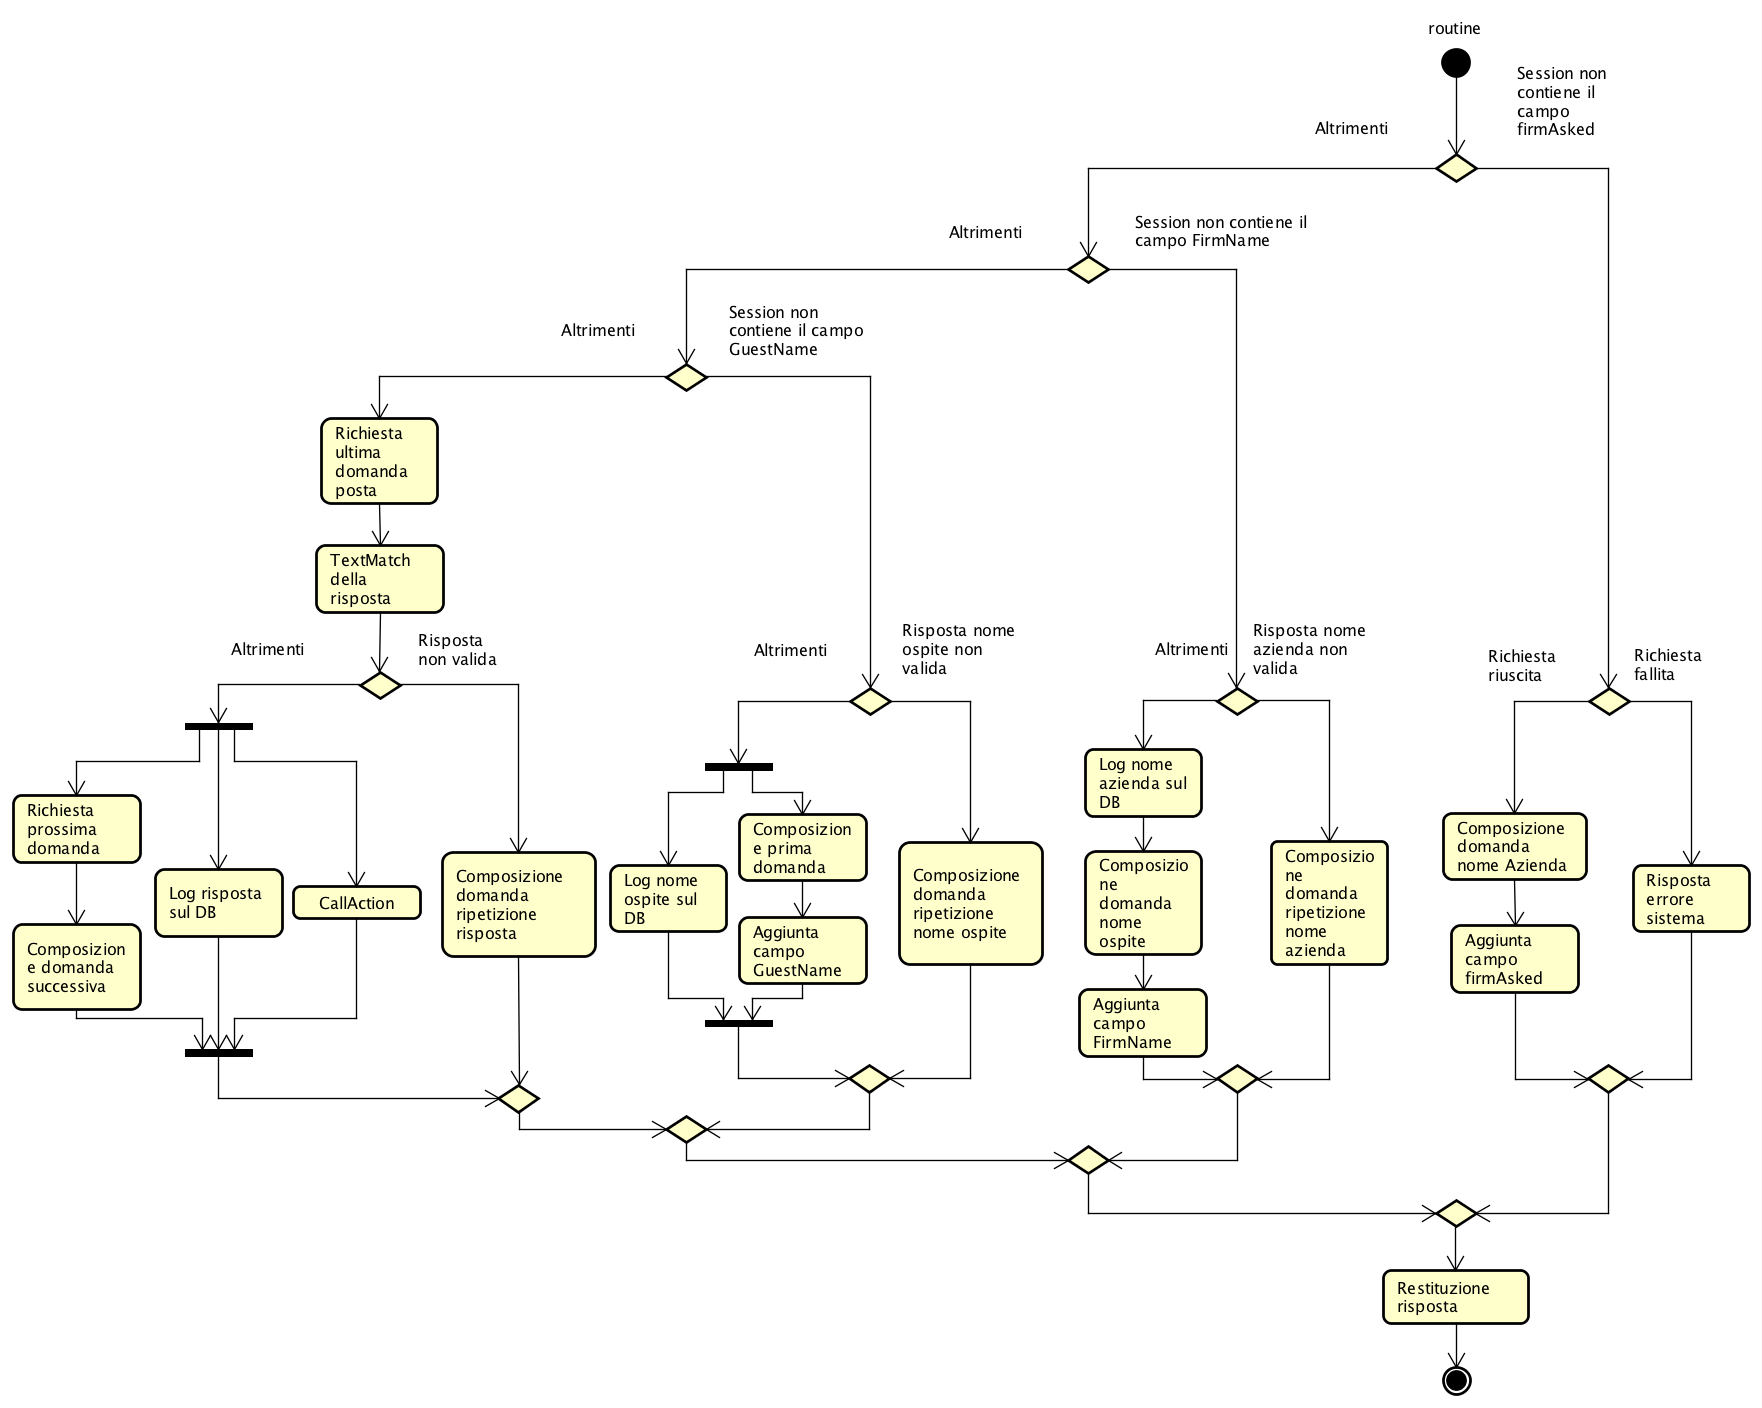
\includegraphics[scale=0.7]{DiagrammiFlusso/FlussoFlowModule.png}
	\caption{Diagramma di attività - \texttt{FlowModule}}
\end{figure}
\begin{description}
	\item [Descrizione] Il diagramma di attività inizia con la verifica, da parte dell'AV, se è presente on oggetto question nel campo \texttt{lastQuestion} della sessione; se non presente l'AV identifica di trovarsi nel caso della prima interazione con l'ospite, imposta il \texttt{sessionId} nella sessione e ottiene la prima domanda da porre.\\Nel caso \texttt{lastQuestion} sia presente viene eseguito il matching della risposta data dall'utente con quelle disponibili. Una volta trovata la risposta corretta viene eseguito il log di quest'ultima richiamata l'esecuzione delle actions ad essa legate.\\
	Successivamente viene controllata la presenza del campo \texttt{id\_nextQuestion}; se non presente viene composta la fine della conversazione, altrimenti si procede a richiedere la \texttt{question} identificata da tale id al database.\\
	Una volta ottenuta la prossima \texttt{question} ne si esegue la \texttt{questionAction} legata, se presente, infine si compone il messaggio della domanda.
\end{description}

\end{document}
